\documentclass{experimento}

\begin{document}

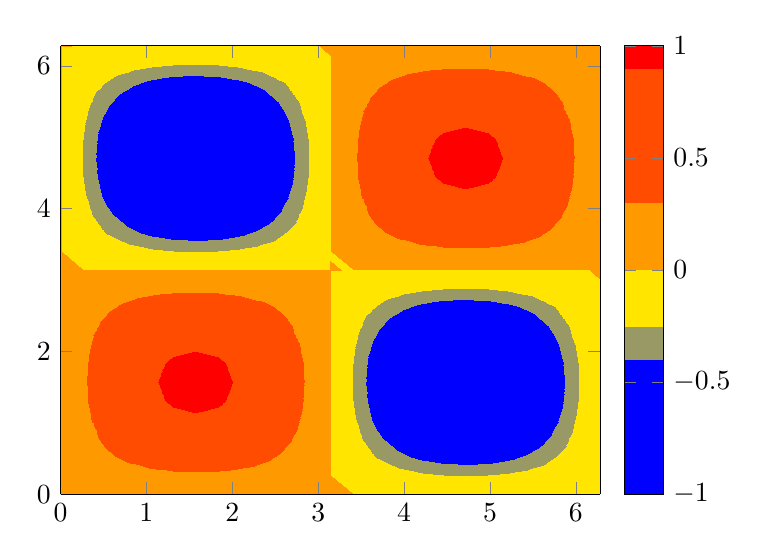
\begin{tikzpicture}
  \begin{axis}[colorbar, view={0}{90}]
  \addplot3 [domain=0:2*pi,trig format plots=rad,
  contour filled={
  levels={-0.4,-0.25,0,0.3,0.9}
  },
  ] {sin(x)*sin(y)};
  \end{axis}
\end{tikzpicture}

\begin{tikzpicture}
  \begin{axis}[view={0}{90}]
    \addplot3 [
      mesh/rows=400,  % Adjust based on your data resolution
      mesh/cols=40,  % Adjust based on your data resolution
      surf,
      shader=interp,
  ] table {mandelbrot_q01.data};
  \end{axis}
\end{tikzpicture}

\begin{tikzpicture}
  \begin{axis}[
      xlabel={Re($c$)},
      ylabel={Im($c$)},
      xmin=-2, xmax=1,
      ymin=-1.5, ymax=1.5,
      colormap={blackwhite}{
        color(0)=(black)
        color(1)=(white)
      },
      colorbar,
      colorbar style={
        ylabel={Escape rate},
        ytick={0,0.2,0.4,0.6,0.8,1},
      },
      scatter/use mapped color={
          draw=mapped color,
          fill=mapped color
      },
      point meta min=0,
      point meta max=1
  ]

  % Plot points as tiny squares
  \addplot[
      only marks,
      mark size=0.01pt,  % Adjust size of pixels here
      scatter,
      mark=square*,   % Use filled squares as markers
  ] table[point meta=\thisrow{z}] {mandelbrot_q01.data};

  \end{axis}
  \end{tikzpicture}

\end{document}